% Created 2012-05-25 Fri 12:20
\documentclass[compress, 9pt]{beamer}
\usepackage[utf8]{inputenc}
\usepackage[T1]{fontenc}
\usepackage{fixltx2e}
\usepackage{graphicx}
\usepackage{longtable}
\usepackage{float}
\usepackage{wrapfig}
\usepackage{soul}
\usepackage{textcomp}
\usepackage{marvosym}
\usepackage{wasysym}
\usepackage{latexsym}
\usepackage{amssymb}
\tolerance=1000
\usetheme{default}
\usecolortheme[RGB={0,38,93}]{structure}
\usefonttheme{serif}
\useinnertheme{circles}
\useoutertheme[]{shadow}
\setbeamertemplate{navigation symbols}{}
\usepackage{natbib}
\usepackage{fleqn}
\usepackage{epsf}
\usepackage[dvips]{color}
\usepackage{bibentry}
\institute{Computer Science and Engineering \\ University of Michigan}
\providecommand{\alert}[1]{\textbf{#1}}

\title{Real World Planning}
\author{Shiwali Mohan}
\date{\today}
\hypersetup{
  pdfkeywords={},
  pdfsubject={},
  pdfcreator={Emacs Org-mode version 7.8.09}}

\begin{document}

\maketitle

\begin{frame}
\frametitle{Outline}
\setcounter{tocdepth}{3}
\tableofcontents
\end{frame}


\title[Search \hspace{1em}\insertframenumber/
\inserttotalframenumber]{Full Title}

\section{Real World Planning}
\label{sec-1}
\begin{frame}
\frametitle{Review}
\label{sec-1-1}

\begin{itemize}
\item Classical Planning
\begin{itemize}
\item fully observable
\item deterministic
\item finite
\item static
\item discrete
\end{itemize}
\end{itemize}
\end{frame}
\begin{frame}
\frametitle{Review}
\label{sec-1-2}
\begin{itemize}

\item (non) Classical Planning (for uncertainty)
\label{sec-1-2-1}%
\begin{itemize}
\item \st{fully observable} partially observable
\item \st{deterministic} non deterministic
\item finite
\item static
\item discrete
\end{itemize}

\item <2-> Approaches
\label{sec-1-2-2}%
\begin{itemize}
\item Sensorless Planning
\item Conditional Planning
\item Execution Monitoring and Replanning
\item Uncertainty Modeling
\end{itemize}
\end{itemize} % ends low level
\end{frame}
\begin{frame}
\frametitle{Weighty Tower of Hanoi}
\label{sec-1-3}
\begin{columns}
\begin{column}{0.6\textwidth}
%% Facts
\label{sec-1-3-1}
\begin{itemize}

\item <1-> Similar to regular Tower of Hanoi
\label{sec-1-3-1-1}%
\begin{itemize}

\item disk are to be ordered by their weight
\label{sec-1-3-1-1-1}%

\item \texttt{clear(), on(), smaller(), disk()}
\label{sec-1-3-1-1-2}%

\item <2-> \texttt{clear(), on()}, \st{smaller()} \underline{lighter()}, \texttt{disk()}
\label{sec-1-3-1-1-3}%
\end{itemize} % ends low level

\item <3-> Initial state\\
\label{sec-1-3-1-2}%
\texttt{on(Red, Green), on(Green, Blue)},
  \texttt{on(Blue, A), clear(Red), disc(Red), disc(Green), disk(Blue)}
  \texttt{clear(B), clear(C), lighter(Red, A), lighter(Red, B)} \ldots{}
\end{itemize} % ends low level
\end{column}
\begin{column}{0.5\textwidth}
%% toh
\label{sec-1-3-2}

 \begin{figure}[htb]
 \centering
 \includegraphics[width=4cm]{../images/newtoh.eps}
 \caption{objects: disks - red, green, blue; pegs - A, B, C}
 \end{figure}
\end{column}
\end{columns}
%% Action
\label{sec-1-3-3}
\begin{itemize}

\item <4-> Action\\
\label{sec-1-3-3-1}%
\texttt{Action(move(disk, source, destination)}\\
             \texttt{PRECOND: clear(disk) \textasciicircum{} on(disk, source) \textasciicircum{} clear(destination)}
    \texttt{\textasciicircum{}lighter(disk,destination)}\\
             \texttt{EFFECT: on(disk, destination) \textasciicircum{} -on(disk, source) \textasciicircum{} -clear(destination) \textasciicircum{}clear(source)}

\end{itemize} % ends low level
\end{frame}
\begin{frame}
\frametitle{Weighty Tower of Hanoi}
\label{sec-1-4}
\begin{itemize}

\item <1-> Can we do sensorless planning?
\label{sec-1-4-1}%

\item <2-> How would the agent do conditional planning?
\label{sec-1-4-2}%

\item <3-> Percept Schema\\
\label{sec-1-4-3}%
\texttt{Percept(lighter(d1,d2)}\\
   \texttt{PRECOND: disk(d1) \textasciicircum{} disk(d2) \textasciicircum{} comparing(d1,d2))}

\item <4-> Information-gathering Action\\
\label{sec-1-4-4}%
\texttt{Action(compare-weight(d1,d2)}\\
   \texttt{PRECOND: disk(d1) \textasciicircum{} disk(d2) \textasciicircum{} clear(d1) \textasciicircum{} clear(d2)}\\
   \texttt{EFFECT: comparing(d1,d2))}

\end{itemize} % ends low level
\end{frame}
\begin{frame}
\frametitle{Slippery Tower of Hanoi}
\label{sec-1-5}
\begin{columns}
\begin{column}{0.5\textwidth}
%% Facts
\label{sec-1-5-1}
\begin{itemize}

\item <1-> Similar to regular Tower of Hanoi
\label{sec-1-5-1-1}%
\begin{itemize}
\item \texttt{clear(), on(), smaller(), disk()}
\item the gripper is slippery. sometimes the disk is displaced to the
    destination but at others it remains at the source.
\end{itemize}

\item <2-> Initial state?
\label{sec-1-5-1-2}%

\item <3-> Goal State?
\label{sec-1-5-1-3}%
\end{itemize} % ends low level
\end{column}
\begin{column}{0.5\textwidth}
%% toh
\label{sec-1-5-2}

\begin{figure}[htb]
\centering
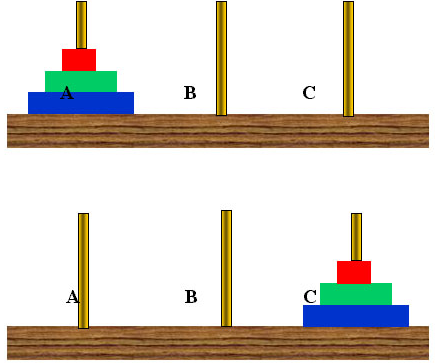
\includegraphics[width=5cm]{../images/torrehanoi.png}
\caption{objects: disks - red, green, blue; pegs - A, B, C}
\end{figure}
\end{column}
\end{columns}
%% Action
\label{sec-1-5-3}
\begin{itemize}

\item <4-> Action\\
\label{sec-1-5-3-1}%
\texttt{Action(move(disk, source, destination)}\\
             \texttt{PRECOND: clear(disk) \textasciicircum{} on(disk, source) \textasciicircum{} clear(destination)     \textasciicircum{}smaller(disk,destination)}\\
             \texttt{EFFECT: (on(disk, destination) \textasciicircum{} -on(disk, source) \textasciicircum{}}
             \texttt{-clear(destination) \textasciicircum{}clear(source)) V (on(disk, source))}
\end{itemize} % ends low level
\end{frame}
\section{SGP Demo}
\label{sec-2}

\end{document}
